\documentclass[dvisvgm,border=0pt]{standalone}
\usepackage[T1]{fontenc}
\usepackage{newtxtext,newtxmath}
\usepackage{tikz}
\usetikzlibrary{arrows.meta,decorations.pathmorphing}

\definecolor{Navy}{HTML}{08154F}
\definecolor{Ink}{HTML}{2B5098}
\definecolor{Blue}{HTML}{315EDB}
\definecolor{BlueTint}{HTML}{DCEBFC}
\definecolor{Sage}{HTML}{568638}
\definecolor{SageTint}{HTML}{E7F2E1}
\definecolor{Gold}{HTML}{F3B122}
\definecolor{Ice}{HTML}{F3FAFF}
\definecolor{Rule}{HTML}{CAE1FA}
\definecolor{Muted}{HTML}{8B95AA}

\tikzset{
  state/.style={draw=Blue,fill=BlueTint,line width=3bp,rounded corners=10bp},
  operation/.style={draw=Sage,fill=SageTint,line width=3bp,rounded corners=10bp},
  wire/.style={draw=Blue,line width=3bp,line cap=round,line join=round},
  blue arrow/.style={wire,-{Stealth[length=13bp,width=12bp]}},
  gold arrow/.style={draw=Gold,line width=6bp,line cap=round,-{Stealth[length=19bp,width=20bp]}},
  time arrow/.style={draw=Muted,line width=3bp,-{Stealth[length=17bp,width=15bp]}},
}

\newcommand{\figbackground}[2]{
  \path[use as bounding box] (0,0) rectangle (#1,#2);
  \fill[Ice!45] (0,0) rectangle (#1,#2);
}

\newcommand{\figtext}[5][Navy]{
  \node[text=#1,font=\fontsize{#4}{#4}\selectfont,inner sep=0bp,align=center]
    at (#2,#3) {#5};
}

\newcommand{\figmath}[5][Navy]{
  \figtext[#1]{#2}{#3}{#4}{$\displaystyle #5$}
}

\newcommand{\panelheading}[3]{
  \fill[BlueTint] (#1,190) circle (35bp);
  \node[text=Navy,font=\fontsize{40}{42}\selectfont\bfseries,inner sep=0bp]
    at (#1,190) {#2};
  \node[text=Navy,anchor=west,font=\fontsize{40}{42}\selectfont\bfseries,inner sep=0bp]
    at ({#1+62},190) {#3};
}

\newcommand{\panelrules}{
  \draw[Rule,line width=2bp] (535,162) -- (535,733);
  \draw[Rule,line width=2bp] (1090,162) -- (1090,733);
}

\newcommand{\statebox}[4]{
  \fill[Blue,opacity=.08,rounded corners=10bp]
    ({#1+4},{#2+6}) rectangle ({#3+4},{#4+6});
  \draw[state] (#1,#2) rectangle (#3,#4);
}

\newcommand{\operationbox}[4]{
  \fill[Sage,opacity=.08,rounded corners=10bp]
    ({#1+4},{#2+6}) rectangle ({#3+4},{#4+6});
  \draw[operation] (#1,#2) rectangle (#3,#4);
}

\newcommand{\processstrip}[4]{
  \fill[BlueTint!70,rounded corners=20bp] (50,762) rectangle (1622,858);
  \foreach \x/\word in {132/#1,522/#2,912/#3,1302/#4} {
    \fill[BlueTint,rounded corners=15bp] (\x,781) rectangle ({\x+306},837);
    \node[text=Navy,font=\fontsize{30}{34}\selectfont\bfseries,inner sep=0bp]
      at ({\x+153},809) {\word};
  }
  \foreach \x in {465,855,1245} {
    \draw[gold arrow] (\x,809) -- ({\x+31},809);
  }
}


\begin{document}
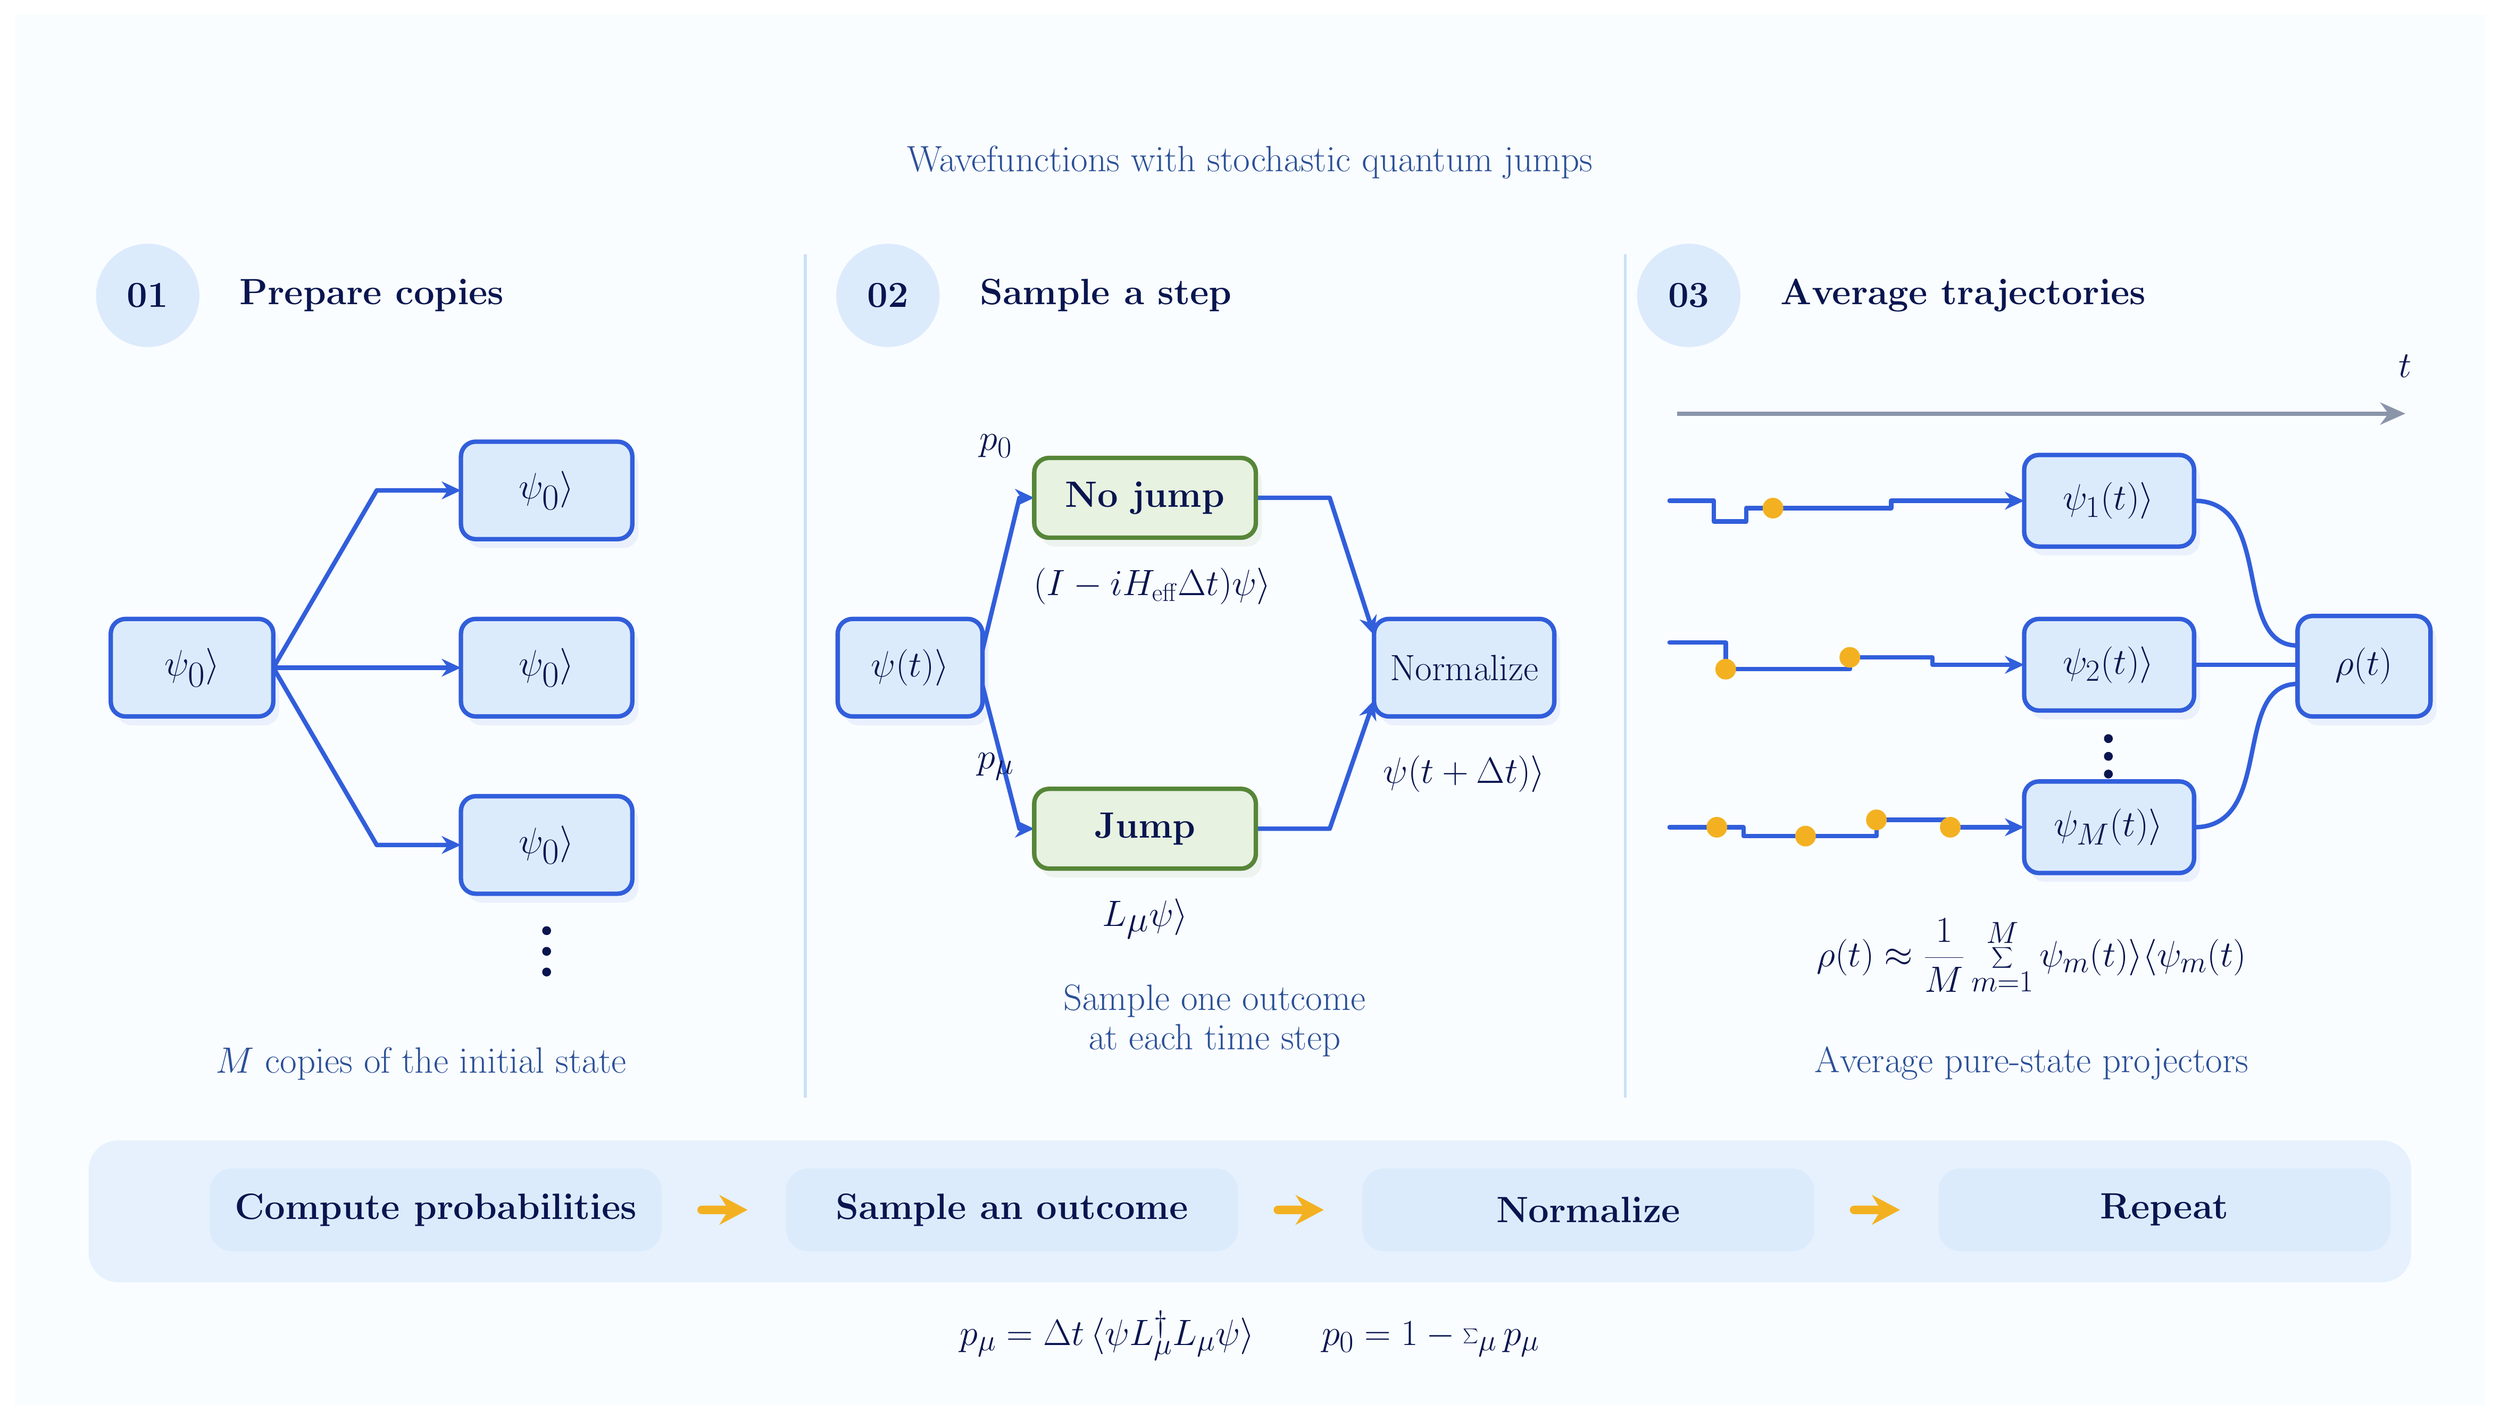
\begin{tikzpicture}[x=1bp,y=-1bp]
  \figbackground{1672}{941}
  \figtext[Ink]{836}{100}{38}{Wavefunctions with stochastic quantum jumps}
  \panelrules
  \panelheading{90}{01}{Prepare copies}
  \panelheading{591}{02}{Sample a step}
  \panelheading{1133}{03}{Average trajectories}

  % Independent copies of the same initial state.
  \draw[blue arrow] (175,442) -- (245,322) -- (302,322);
  \draw[blue arrow] (175,442) -- (302,442);
  \draw[blue arrow] (175,442) -- (245,562) -- (302,562);
  \statebox{65}{409}{175}{475}
  \figmath{120}{442}{36}{\lvert\psi_0\rangle}
  \foreach \y in {322,442,562} {
    \statebox{302}{\y-33}{418}{\y+33}
    \figmath{360}{\y}{36}{\lvert\psi_0\rangle}
  }
  \foreach \y in {620,634,648} {\fill[Navy] (360,\y) circle (3bp);}
  \figtext[Ink]{275}{710}{30}{$M$ copies of the initial state}

  % One categorical outcome is selected at each discrete time step.
  \draw[blue arrow] (655,430) -- (680,327) -- (690,327);
  \draw[blue arrow] (655,454) -- (680,551) -- (690,551);
  \draw[blue arrow] (840,327) -- (890,327) -- (920,420);
  \draw[blue arrow] (840,551) -- (890,551) -- (920,464);
  \statebox{557}{409}{655}{475}
  \figmath{606}{442}{31}{\lvert\psi(t)\rangle}
  \operationbox{690}{300}{840}{354}
  \operationbox{690}{524}{840}{578}
  \figtext{765}{327}{31}{\textbf{No jump}}
  \figtext{765}{551}{31}{\textbf{Jump}}
  \figmath{664}{292}{31}{p_0}
  \figmath{664}{509}{31}{p_\mu}
  \figmath{770}{387}{25}{(I-iH_{\mathrm{eff}}\Delta t)\lvert\psi\rangle}
  \figmath{765}{612}{34}{L_\mu\lvert\psi\rangle}
  \statebox{920}{409}{1042}{475}
  \figtext{981}{442}{25}{Normalize}
  \figmath{981}{514}{27}{\lvert\psi(t+\Delta t)\rangle}
  \figtext[Ink]{812}{681}{27}{Sample one outcome\\at each time step}

  % Schematic histories, not plotted observables or numerical data.
  \draw[time arrow] (1125,270) -- (1618,270);
  \figmath{1618}{238}{35}{t}
  \draw[blue arrow] (1120,329) -- (1150,329) -- (1150,343) --
    (1172,343) -- (1172,334) -- (1270,334) -- (1270,329) -- (1360,329);
  \draw[blue arrow] (1120,425) -- (1158,425) -- (1158,443) --
    (1242,443) -- (1242,435) -- (1298,435) -- (1298,440) -- (1360,440);
  \draw[blue arrow] (1120,550) -- (1170,550) -- (1170,556) --
    (1260,556) -- (1260,545) -- (1310,545) -- (1310,550) -- (1360,550);
  \foreach \x/\y in {1190/334,1158/443,1242/435,1152/550,1212/556,1260/545,1310/550} {
    \fill[Gold] (\x,\y) circle (7bp);
  }
  \draw[wire] (1475,329) .. controls (1530,329) and (1500,427) .. (1545,427);
  \draw[wire] (1475,440) -- (1545,440);
  \draw[wire] (1475,550) .. controls (1530,550) and (1500,453) .. (1545,453);
  \foreach \y/\m in {329/1,440/2,550/M} {
    \statebox{1360}{\y-31}{1475}{\y+31}
    \figmath{1417}{\y}{30}{\lvert\psi_{\m}(t)\rangle}
  }
  \foreach \y in {490,502,514} {\fill[Navy] (1417,\y) circle (3bp);}
  \statebox{1545}{407}{1635}{475}
  \figmath{1590}{441}{34}{\rho(t)}
  \figmath{1365}{637}{31}{
    \rho(t)\approx\frac{1}{M}\sum_{m=1}^{M}
    \lvert\psi_m(t)\rangle\langle\psi_m(t)\rvert
  }
  \figtext[Ink]{1365}{710}{29}{Average pure-state projectors}

  \processstrip{Compute probabilities}{Sample an outcome}{Normalize}{Repeat}
  \figmath{836}{894}{29}{
    \textstyle p_\mu=\Delta t\,\langle\psi\rvert L_\mu^\dagger L_\mu\lvert\psi\rangle
    \qquad p_0=1-\sum_\mu p_\mu
  }
\end{tikzpicture}
\end{document}
